\documentclass[12 pt]{article}
\usepackage{easycalc3}
\usepackage{setspace}
\usepackage{enumerate}
\usepackage{lastpage}
\usepackage{float}
\usepackage{fancyhdr}
\usepackage{tikz}
\usepackage{tabularx}
\usepackage{ltablex}
\usepackage{textcomp}
\usepackage[T1]{fontenc}
\usepackage{listings}
\usepackage[margin=1 in]{geometry}
\allowdisplaybreaks
%\usepackage[dvipsnames]{xcolor}   %May be necessary if you want to color links
\usepackage{graphicx}
\graphicspath{{images/}}
\author{Sarah Randall}
\date{Last updated: \today}
\title{MATH 222: Week 3}
\pagestyle{fancy}
\lhead{MATH 222}
\chead{\leftmark}
\rhead{Sarah Randall}
\cfoot{Page \thepage \ of \pageref{LastPage}}
\newcommand{\tab}[1]{\hspace{.2\textwidth}\rlap{#1}}
\begin{document}
    \onehalfspacing
    \maketitle
    \tableofcontents
    \section{\S 13.3 Arc Length + Curvature}
        \subsection{Arc Length}
        Given a parametric curve $\vec{r}(t)$ in $\R^3$, what is the distance travelled by the particle between some $t=a$ and $t=b$?

        Suppose we partition this section of the curve into $n$ sections of time. The differences in $t$ between these sections might not be 1 so we write $\Delta t=\frac{b-a}{n}$. In this way $b$ would equal $a+n\Delta t$. We could approximate the distance from $\vec{r}(a)$ to $\vec{r}(b)$ by adding together these the difference between $\vec{r}(a)$ and $\vec{r}(a+\Delta t)$, $\vec{r}(a+\Delta t)$ and $\vec{r}(a+2\Delta t)$, and so on. If we had three sections, the approximation would look something like this:
        $$\sum_{i=0}^2\sqrt{(x(a+(i+1)\Delta t)-x(a+(i)\Delta t))^2+(y(a+(i+1)\Delta t)-y(a+(i)\Delta t))^2}$$\\

        I'll cut this short, but we can basically turn this into a Riemann sum by having $n$ approach infinity. Then by using the Mean Value Theorem, we can find an actual equation for Arc Length (here denoted by $L$):
        $$L=\int_a^b \sqrt{(x'(t))^2+(y'(t))^2}\ dt$$
        The professor has included more notes about how this is derived on MyCourses, so check that out if you're really, really, really interested for some reason.

        For some $\vec{r}(t)=<f(t),g(t),h(t)>$ in $\R^3$, the formula is slightl different. We just need to add the third function.
        $$L=\int_a^b \sqrt{(f'(t))^2+(g'(t))^2+(h'(t))^2}\ dt$$
        This is also written as
        $$L=\int_a^b\parallel \vec{r'}(t)\parallel\ dt$$

        \begin{exmp*}
            Compute arc length over $0\leq t\leq2\pi$ of the circular helix $\vec{r}(t)=<\cos{t},\sin{t},t>$

            Find $\vec{r'}(t)$ and its length
            $$\vec{r'}(t)=<-\sin{t},\cos{t},1>$$
            $$\parallel\vec{r'}(t)\parallel=\sqrt{(\sin(t))^2+(\cos(t))^2+1}=\sqrt{2}$$

            Then integrate this
            $$\int_0^{2\pi}\sqrt{2}\ dt=2\pi\sqrt{2}-0\sqrt{2}=2\pi\sqrt{2}$$
        \end{exmp*}

        \subsection{Curvature}

        Suppose we are on some interval of $t$ where $\vec{r}(t)$ is a smooth function and $\vec{r'}(t)\neq 0$. In this setting we can discuss the curvature of the curve defined by $\vec{r}(t)$.

        We think of curvature as the amount that the direction of the curve changes over a small step (the size of this step approaches 0)

        Curvature depends solely on arc length. $<\cos(t),\sin(t)>$ is "drawn" more slowly than $<\cos(4t),\sin(4t)$ but they still have the same curvature because they're both circles with the same radius. We can define curvature as the rate of change of the unit tangent vector with respect to arc length, which would be written as this (where $K(t)$ is curvature at time $t$):
        \begin{align*}
            K(t)&=\parallel\frac{d\vec{T}}{ds}\parallel\\
            &=\parallel\frac{d\vec{T}}{dt}\frac{dt}{ds}\parallel\\
            &=\parallel\frac{d\vec{T}}{dt}\frac{1}{\parallel\vec{r'}(t)\parallel}\parallel\\
        \end{align*}
        In the last line we were able to replace $\frac{dt}{ds}$ with $\frac{1}{\parallel\vec{r'}(t)\parallel}$ because the rate in change of $s$ (arc length) with respect to time $t$ is $\parallel\vec{r'}(t)\parallel$ based on our equations for arc length. We just need to invert this to get $\frac{1}{\parallel\vec{r'}(t)\parallel}$.

        By simplifying a bit more ($\frac{d\vec{T}}{dt}=\vec{T'}(t)$), we can write the equation for curvature at time $t$ as
        $$K(t)=\frac{\parallel\vec{T'}(t)\parallel}{\parallel\vec{r'}(t)\parallel}$$

        Through a very long proof we also proved that there is an alternate equations for the curvature that may be easier to use in some cases.
        $$K(t)=\frac{\parallel\vec{r'}(t)\times\vec{r''}(t)\parallel}{\parallel\vec{r'}(t)\parallel^3}$$
        I will show the proof here (the book's much shorter version) but feel free to skip over this.

        \begin{proof}
            $K=\frac{\parallel\vec{r'}(t)\times\vec{r''}(t)\parallel}{\parallel\vec{r'}(t)\parallel^3}$

            Since $\vec{T}=\frac{\vec{r}}{\parallel\vec{r'}\parallel}$ and $\parallel\vec{r'}=\frac{ds}{dt}$, we can write that
            $$\vec{r'}=\parallel\vec{r'}\parallel\vec{T}=\frac{ds}{dt}\vec{T}$$
            Using the product rule we can find that
            $$\vec{r''}=\frac{d^2s}{dt^2}\vec{T}+\frac{ds}{dt}\vec{T'}$$
            Since the equation we wish to achieve has $\vec{r'}\times\vec{r''}$ in it, let's try to see what happens when we take the cross product.
            $$\vec{r'}\times\vec{r''}=\frac{ds}{dt}\vec{T}\times\frac{d^2s}{dt^2}\vec{T}+\frac{ds}{dt}\vec{T}\times\frac{ds}{dt}\vec{T'}$$
            We know that $\vec{T}\times\vec{T}$ will be 0.
            $$\vec{r'}\times\vec{r''}=(\frac{ds}{dt})^2(\vec{T}\times\vec{T'})$$
            Next we will take the magnitude of both sides but we can also simplifying the cross product. Since $\parallel \crossp{a}{b}\parallel=\magn{a}\magn{b}\sin{\theta}$ and $\vec{T}$ is perpendicular to $\vec{T'}$, $\theta=\frac{\pi}{2}$. $\sin(\frac{\pi}{2})=1$. Therefore the cross product can be rewritten.
            $$\parallel\vec{r'}\times\vec{r''}\parallel=(\frac{ds}{dt})^2\magn{T}\magn{T'}$$
            $\vec{T}$ is defined to be a unit vector, so its magnitude is 1.
            $$\parallel\vec{r'}\times\vec{r''}\parallel=(\frac{ds}{dt})^2\magn{T'}$$
            Solving for $\magn{T'}$ gives
            $$\magn{T'}=\frac{\parallel\vec{r'}\times\vec{r''}\parallel}{(ds/dt)^2}=\frac{\parallel\vec{r'}\times\vec{r''}\parallel}{\magn{r'}^2}$$
            Finally, if we divide all of this by $\magn{r'}$ in order to get the equation for curvature on one side $\frac{\magn{T'}}{\magn{r'}}$, we can see that our theorem is true.
            $$K(t)=\frac{\magn{T'}}{\magn{r'}}=\frac{\parallel\vec{r'}\times\vec{r''}\parallel}{\magn{r'}^3}$$
            So there are two equivalent ways of finding an equation for curvature.
        \end{proof}
        \begin{exmp*}
            Compute the curvature of $\vec{r}(t)=<t\cos(t),t\sin(t),t>$ at $t=\frac{\pi}{2}$

            We need $\vec{r'}$, $\vec{r''}$, and $\magn{r'}$
            \begin{align*}
                \vec{r'}(t)&=<-t\sin(t)+\cos(t),t\cos(t)+\sin(t),t>\\
                \vec{r'}(\frac{\pi}{2})&=<-\frac{\pi}{2},1,1>\\
                \parallel\vec{r'}(\frac{\pi}{2})\parallel&=\parallel<-\frac{\pi}{2},1,1>\parallel=\sqrt{\frac{\pi^2}{4}+2}\\
                \vec{r''}(t)&=<-t\cos(t)-\sin(t)-\sin(t),-t\sin(t)+\cos(t)+\cos(t),0>\\
                &=<-t\cos(t)-2\sin(t),-t\sin(t)+2\cos(t),0>\\
                \vec{r''}(\frac{\pi}{2})&=<-2,-\frac{\pi}{2},0>
            \end{align*}
            Now that we have all the piece we need, we just plug it all into the curvature equation.\\
            $\vec{r'}(\pi/2)\times\vec{r''}(\pi/2)=
            \begin{vmatrix}
                i & j & k \\
                -\frac{\pi}{2} & 1 & 1 \\
                -2 & -\frac{\pi}{2} & 0
            \end{vmatrix}
            =<\frac{\pi}{2},-2,\frac{\pi^2}{4}+2>$
            Our equation for curvature is therefore
            $$K(\frac{\pi}{2})=\frac{\parallel<\frac{\pi}{2},-2,\frac{\pi^2}{4}+2>\parallel}{(\frac{\pi^2}{4}+2)^{3/2}}=\frac{\sqrt{\frac{\pi^2}{4}+4+(\frac{\pi^2}{4}+2)^2}}{(\frac{\pi^2}{4}+2)^{3/2}}$$
            You can do the insane amount of computation if you'd like, but it's sufficient to just plug this into a calculator.
        \end{exmp*}

        \subsection{Curvature of functions}

        The concept of curvature can also be applied to functions $y=f(x)$ since a parametrization of a function like this is $\vec{r}(x)=<x,f(x),0>$
        $$\vec{r'}(x)=<1,f'(x),0>$$
        $$\vec{r''}(x)=<0,f''(x),0>$$
        $\vec{r'}(x)\times\vec{r''}(x)=
        \begin{vmatrix}
            i & j & k \\
            1 & f'(x) & 0 \\
            0 & f''(x) & 0
        \end{vmatrix}
        =k(f''(x))$
        Therefore $\parallel\vec{r'}\times\vec{r''}\parallel=\lvert f''(x)\rvert$. The curvature of any function $y=f(x)$ can be written as
        $$K(x)=\frac{\lvert f''(x)\rvert}{(1+(f'(x))^2)^{3/2}}$$
        \begin{exmp*}
            Find $K(x)$ for $f(x)=x^2$

            $f'(x)=2x$ and $f''(x)=2$. Therefore $K(x)$ is
            $$K(x)=\frac{2}{(1+4x^2)^{3/2}}$$
        \end{exmp*}

        \subsection{Normal and Binormal Vectors}

        Earlier we learned that $\vec{T}(t)\cdot\vec{T'}(t)=0$, which implies that the two vectors are perpendicular.

        Let $\vec{N}(t)=\frac{\vec{T'}(t)}{\parallel\vec{T'}(t)\parallel}$. We call this the "unit outward normal". $N(t)$ indicates the direction in which the curve given by $\vec{r}(t)$ is turning.

        In addition, let $\vec{B}(t)=\vec{T}(t)\times\vec{N}(t)$. We call this the binormal vector. Since $\vec{B}(t)$ is orthogonal to both $\vec{T}(t)$ and $\vec{N}(t)$ and these vectors are in the same plane, $\vec{B}(t)$ comes "out" of the page and is orthogonal to that plane.

        Vectors $B$ and $N$ form the normal plane to curve $C$ at point $P$ where $t=a$. The normal plane contains all vectors that are perpendicular to $T$.
        Vectors $T$ and $N$ form the osculating plane to curve $C$ at point $P$. The osculating plane contains all vectors that are perpendicular to $B$.

        \begin{exmp*}Find the equation for the normal plane at $t=\frac{\pi}{2}$ for $\vec{r}(t)=<\cos(t),\sin(t),t^2>$

            $$\vec{T}=\frac{r'}{\magn{r'}}=\frac{<-\sin(t),\cos(t),2t>}{\sqrt{1+4t^2}}$$
            $$\vec{T}(\frac{\pi}{2})=\frac{<-1,0,\pi>}{\sqrt{1+\pi^2}}$$
            Since $\vec{T}$ is the normal to our plane, we can find the equation of this plane using $\vec{n}\cdot(\vec{r}-\vec{r_0})=0$.
            $$\frac{1}{\sqrt{1+\pi^2}}<-1,0,\pi>\cdot((x,y,z)-(0,1,\frac{\pi^2}{4}))=0$$
            $$\frac{-1}{\sqrt{1+\pi^2}}(x)+\frac{\pi}{\sqrt{1+\pi^2}}(z-\frac{\pi^2}{4})=4$$
            This is the equation of the normal plane to the curve at $t=\frac{\pi}{2}$.
        \end{exmp*}
    \section{\S 13.4 Acceleration Vector}
        If $\vec{r}(t)$ denotes position, $\vec{r'}(t)=\vec{v}(t)$ denotes the velocity vector. Also, $\vec{r''}(t)=\vec{a}(t)$ denotes the acceleration vector.

        The magnitude of the velocity vector is speed, and it is written as $\nu(t)$

        Since $\vec{a}(t)=\vec{v}(t)$, then
        $$\int_{t_0}^t\vec{a}(\tau)\ d\tau=\int_{t_0}^t\vec{v'}(\tau)\ d\tau=\vec{v}(t)-\vec{v}(t_0)$$
        $$\vec{v}(t)=\vec{v}(t_0)+\int_{t_0}^t\vec{a}(\tau)\ d\tau$$
        If we can integrate $\vec{a}(t)$ and we have the initial velocity, we can find $\vec{v}(t)$

        \subsection{Tangential and normal components of acceleration}

        It is often useful to be able to break up the acceleration vector into its components. We'll start with the definition of $\vec{T}(t)$.
        $$\vec{T}=\frac{\vec{r'}}{\magn{r'}}=\frac{\vec{v}}{\magn{v}}=\frac{\vec{v}}{\nu}$$
        From here we can see that
        $$\vec{v}=\nu\vec{T}$$
        If we differentiate both sides of this with respect to $t$, we get that
        $$\vec{a}=\vec{v'}=\nu'\vec{T}+\nu\vec{T'}$$
        Using the equation for curvature and replacing $\magn{r'}$ with $\nu$, we can solve for $\magn{T'}$ and get $\magn{T'}=K\nu$. We can substitute this into the equation for $\vec{N}$ and see that
        $$\vec{N}=\frac{\vec{T'}}{\magn{T'}}$$
        $$\vec{T'}=\vec{N}\magn{T'}$$
        Substituting this into the equation we were originally working on gives
        $$\vec{a}=\nu'\vec{T}+K\nu\vec{N}$$
        We are able to write $\vec{a}$ as a combintion of a scalar multiple of the unit tangent and a scalar multiple of the unit normal. When talking about the components of the acceleration vector, we call the component in the direction of $\vec{T}$ $a_T$, which equals $\nu'$. The component in the direction of $\vec{N}$ is called $a_N$ and it equals $K\nu^2$.

        One interesting thing that this information implies is that the acceleration vector will always be in the osculating plane, since $\vec{B}$ is not one of the components of $\vec{a}$.

        For convenience sake, since we'll often be computing $\vec{r},\ \vec{r'},\ \vec{r''}$ it would be nice to have equations for these components in terms of these vectors. The book goes into more deal why they do what they do to derive these equations, but here they are:
        $$a_T=\frac{\vec{r'}(t)\cdot\vec{r''}(t)}{\parallel\vec{r'}(t)\parallel}$$
        $$a_N=\frac{\parallel\vec{r'}(t)\times\vec{r''}(t)\parallel}{\parallel\vec{r'}(t)\parallel}$$

    \section{\S 14.1 Multivariable Functions}
        \begin{def*}
            A function of two variables is a rule that assigns to each ordered pair $(x,y)$ in a set $D$ the unqiue real number $f(x,y)$. We write that $z=f(x,y)$
        \end{def*}
        The domain of $f(x,y)$ is the set of all $x,y)\in\R^2$ where $f(x,y)$ is a well-defined real number. This means that $f(x,y)$ cannot output nothing nor can it output more than one value (For those who have taken Linear Algebra 2 or Discrete Mathematics, our function must be injective and surjective).

        \begin{exmp*}
            Find the domains of the functions $f(x,y)=\sqrt{xy}$ and $f(x,y)=\ln(y-x^2+1)$.

            For the first function, $\sqrt{xy}$ will have non-real output if $xy$ is negative. This means we either need both $x$ and $y$ to be positive or negative. Therefore the domain of this function is $x\geq 0,\ y\geq 0$ and $x\leq 0,\ y\leq 0$.

            For the second function, we can't have the natural log of a negative number because there is no number $n$ such that $e^n$ is a negative number. This means we need $y-x^2+1\geq 0$. Slightly rewriting this gives the domain as $y\geq x^2-1$, which is a parabola. To help visualiza this, a quick test tells us that $(0,2)$ will gives us real output for this function but $(0,-2)$ will not. This implies that since this parabola is concave up, any value of $(x,y)$ on or above the parabola is in the domain of the function.
        \end{exmp*}

        \begin{def*}
            We say that the graph of a function with 2 variables is the set of all $(x,y,z)\in\R^3$ such that $z=f(x,y)$ for all $(x,y)$ in the domain of the function.
        \end{def*}

        \subsection{Level Curves}

        \begin{def*}
            The level curves of a function $z=f(x,y)$ are the curves with equation $k=f(x,y)$ for some constant $k$ in the range of $f(x,y)$. Essentially, we are finding all $(x,y)$ points that make $z=k$. Drawings of the level curves of a function will look sort of like a layer cake.
        \end{def*}
        A good example given in class of level curves is a contour map, where each line represents a certain elevation. Level curves can be useful for quickly getting a general shape of a function by finding a few of its level curves. We will be using level curves more in the future.
    \section{\S 14.2 Limits and Continuity}
        \begin{def*}
            Let $f$ be a function of 2 variables with domain $D$ that includes a "neighborhood" around the point $(a,b)$. We say that the limit of $f(x,y)$ as $(x,y)$ appraoches $(a,b)$ is $L$, written as
            $$\Lim{x,y\rightarrow a,b}f(x,y)=L$$
            if for every number $\varepsilon>0$ there is a corresponding number $\delta>0$ such that if $(x,y)$ is in the domain D and $0<\sqrt{(x-a)^2+(y-b)^2}<\delta$ (the distance between $(x,y)$ and $(a,b)$ is greater than zero and less than $\delta$), then $\lvert f(x,y)-L\rvert<\varepsilon$.
        \end{def*}

        This sounds pretty obtuse (and it is) so let's try to understand this definition a little better.

        Say we have the following surface which is given by $z=sin(y)+sin(x)$:
        \begin{figure}[!h]
            \centering
            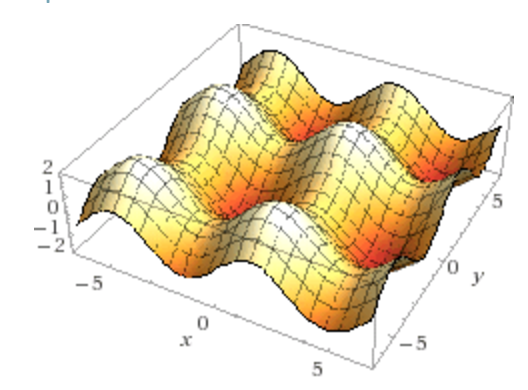
\includegraphics{z=sin(y)+sin(x).png}
        \end{figure}

        The limits of all points on this surface exist because there are no "ledges" on the surface that would create single-sided limits that don't agree.

        I couldn't find any extreme images of a function where a limit would not exist, but image a function that results in two flat surfaces at different elevations. If a point $(a,b)$ were on the edge of one of these surfaces just before the elevation change, the limit would not exist at $(a,b)$. Appraoching $(a,b)$ from the direction of the surface with higher elevation would gives one limit and approaching from the other would gives another limit.

        \subsection{Proving DNE}

        In order to prove this kind of limit exists, we need to prove that the limit of $f(x,y)$ as $(x,y)$ approaches $(a,b)$ is the same no matter the direction in which you approach $(a,b)$. Like all "for all" proofs, it is harder to prove that the limit exists than it is to prove that the limit does not exist. To prove it doesn't exist we just need to find two paths to $(a,b)$ that result in different limits.

        We can test for DNE by substituting $y$ or $x$ with different values or functions, and then finding the limit of the resulting single-variable function. Some common substitutions to make are $y=0$, $x=0$, $y=x$, $y=x^2$. These would, respectively, check the limit on the x-axis, the y-axis, the line $y=x$, and the parabola $y=x^2$. An easy way to test a lot of paths is by substituting $y=mx$, the general equation of a line. If $m$ cannot be removed entirely from the expression, this implies that the limit depends on the direction from which $(a,b)$ is approached. Therefore the limit doesn't exist.

        \begin{exmp*}
            Show that $\Lim{x,y\rightarrow 0,0}\frac{x^2-y^2}{x^2+y^^4}$ does not exist.

            Let $y=mx$

            $$\Lim{x,mx\rightarrow 0,0}\frac{x^2-m^2x^2}{x^2+m^2x^2}=\Lim{x,mx\rightarrow 0,0}\frac{1-m^2}{1+m^2}$$
            We cannot get rid of the $m$. Therefore the limit does not exist because the limit depends on the direction you appraoch $(0,0)$
        \end{exmp*}

        \subsection{Proving limits exist}

        The only way we can prove that these limits DO exist in this course is by using polar coordinates. We must take the limits and make the following substitutions:
        $$x=r\cos(\theta),\ y=r\sin(\theta),\ x^2+y^2=r^2$$
        This allows us to check the the limit for all angles of approach, represented by $\theta$.
        \begin{exmp*}
            Using polar coordinates, show that $\Lim{x,y\rightarrow 0,0} \frac{xy^2}{x^2+y^2}=0$

            First, make the polar substitutions.
            $$\Lim{r\rightarrow 0}\frac{r\cos(\theta)r^2\sin^2(\theta)}{r^2}$$
            $$\Lim{r\rightarrow 0}r\cos(\theta)\sin^2(\theta)$$
            We can use the squeeze theorem to evaluate this
            $$-r\leq r\cos(\theta)\sin^2(\theta)\leq r$$
            Since both $-r$ and $r$ are 0 when $r=0$, by the squeeze theorem our limit must also approach zero. Therefore:
            $$\Lim{x,y\rightarrow 0,0}\frac{xy^2}{x^2+y^2}=0$$
        \end{exmp*}
        \begin{def*}A function $f(x,y)$ is continuous at $(x,y)=(a,b)$ if
            $$\Lim{x,y\rightarrow a,b}f(x,y)=f(a,b)$$
        \end{def*}
        There are a few general rules about continuity for certain types of functions. All multivariable polynomials are always continuous, similar to the behavior for single variable polynomials. All multivariable rational functions are continuous only on their domain, where they are not undefined and where they don't output non-real values.
    \section{\S 14.3 Partial Derivatives}
        Recall that in 1D, $f(x)=\Lim{h\rightarrow 0}\frac{f(x+h)-f(x)}{h}$.
        Derivatives tell us the rise over the run as we take infinitely small steps in the $x$ direction.

        We can compute the same quantity for functions of multiple variables, except not ther are more directions in which we can compute the rise over the run.

        For equations of two variables, we can compute the rise over run in both the x direction and the y direction.
        $$f_x=\frac{\partial f}{\partial x}=\Lim{h\rightarrow 0}\frac{f(x+h,y)-f(x,y)}{h}$$
        $$f_y=\frac{\partial f}{\partial y}=\Lim{h\rightarrow 0}\frac{f(x,y+h)-f(x,y)}{h}$$

        We compute these derivatives by treating the variable we aren't differentiating by as a constant.
        \begin{exmp*}
            Find $f_x$ and $f_y$ of $f(x,y)=x^2+y^2+xy+e^{xy}$
            $$f_x=2x+0+y+ye^{xy}=2x+y+ye^{xy}$$
            $$f_y=0+2y+x+xe^{xy}=2y+x+xe^{xy}$$
        \end{exmp*}

        \subsection{Interpretation of Partials}

        We can use partials to find the tangent plane to a point on a surface or curve. Since the derivative of a single variable function gives the slope of the tangent line, the derivatives of two variable functions give the slopes of two tangent lines. These two lines define a plane, and that plane is tangent to the point on the curve where the derivatives were evaluated.
    \section{\S 14.4 Tangent planes, linear approximation}
\end{document}
